%%%%%%%%%%%%%%%%%%%%%%%%%%%%%%%%%%%%%%%%%
% Classicthesis-Styled CV
% LaTeX Template
% Version 1.0 (22/2/13)
%
% This template has been downloaded from:
% http://www.LaTeXTemplates.com
%
% Original author:
% Alessandro Plasmati
%
% License:
% CC BY-NC-SA 3.0 (http://creativecommons.org/licenses/by-nc-sa/3.0/)
%
%%%%%%%%%%%%%%%%%%%%%%%%%%%%%%%%%%%%%%%%%

%----------------------------------------------------------------------------------------
%	PACKAGES AND OTHER DOCUMENT CONFIGURATIONS
%----------------------------------------------------------------------------------------

\documentclass{scrartcl}

\reversemarginpar % Move the margin to the left of the page 

\newcommand{\MarginText}[1]{\marginpar{\raggedleft\itshape\small#1}} % New command defining the margin text style

\usepackage{graphicx}
\usepackage[nochapters]{classicthesis} % Use the classicthesis style for the style of the document
\usepackage[LabelsAligned]{currvita} % Use the currvita style for the layout of the document

\renewcommand{\cvheadingfont}{\LARGE\color{Maroon}} % Font color of your name at the top

\usepackage{hyperref} % Required for adding links	and customizing them
\hypersetup{colorlinks, breaklinks, urlcolor=Maroon, linkcolor=Maroon} % Set link colors

\newlength{\datebox}\settowidth{\datebox}{Winter 2019} % Set the width of the date box in each block

\newcommand{\NewEntry}[3]{\noindent\hangindent=2em\hangafter=0 \parbox{\datebox}{\small \textit{#1}}\hspace{1.5em} #2 #3 % Define a command for each new block - change spacing and font sizes here: #1 is the left margin, #2 is the italic date field and #3 is the position/employer/location field
\vspace{0.5em}} % Add some white space after each new entry

\newcommand{\Description}[1]{\hangindent=2em\hangafter=0\noindent\raggedright\footnotesize{#1}\par\normalsize\vspace{1em}} % Define a command for descriptions of each entry - change spacing and font sizes here

%----------------------------------------------------------------------------------------

\begin{document}

\thispagestyle{empty} % Stop the page count at the bottom of the first page

%----------------------------------------------------------------------------------------
%	NAME AND CONTACT INFORMATION SECTION
%----------------------------------------------------------------------------------------

\begin{cv}{
\spacedallcaps{Andrea Panontin}}\vspace{1.5em} % Your name

%\Description{\MaginText{
%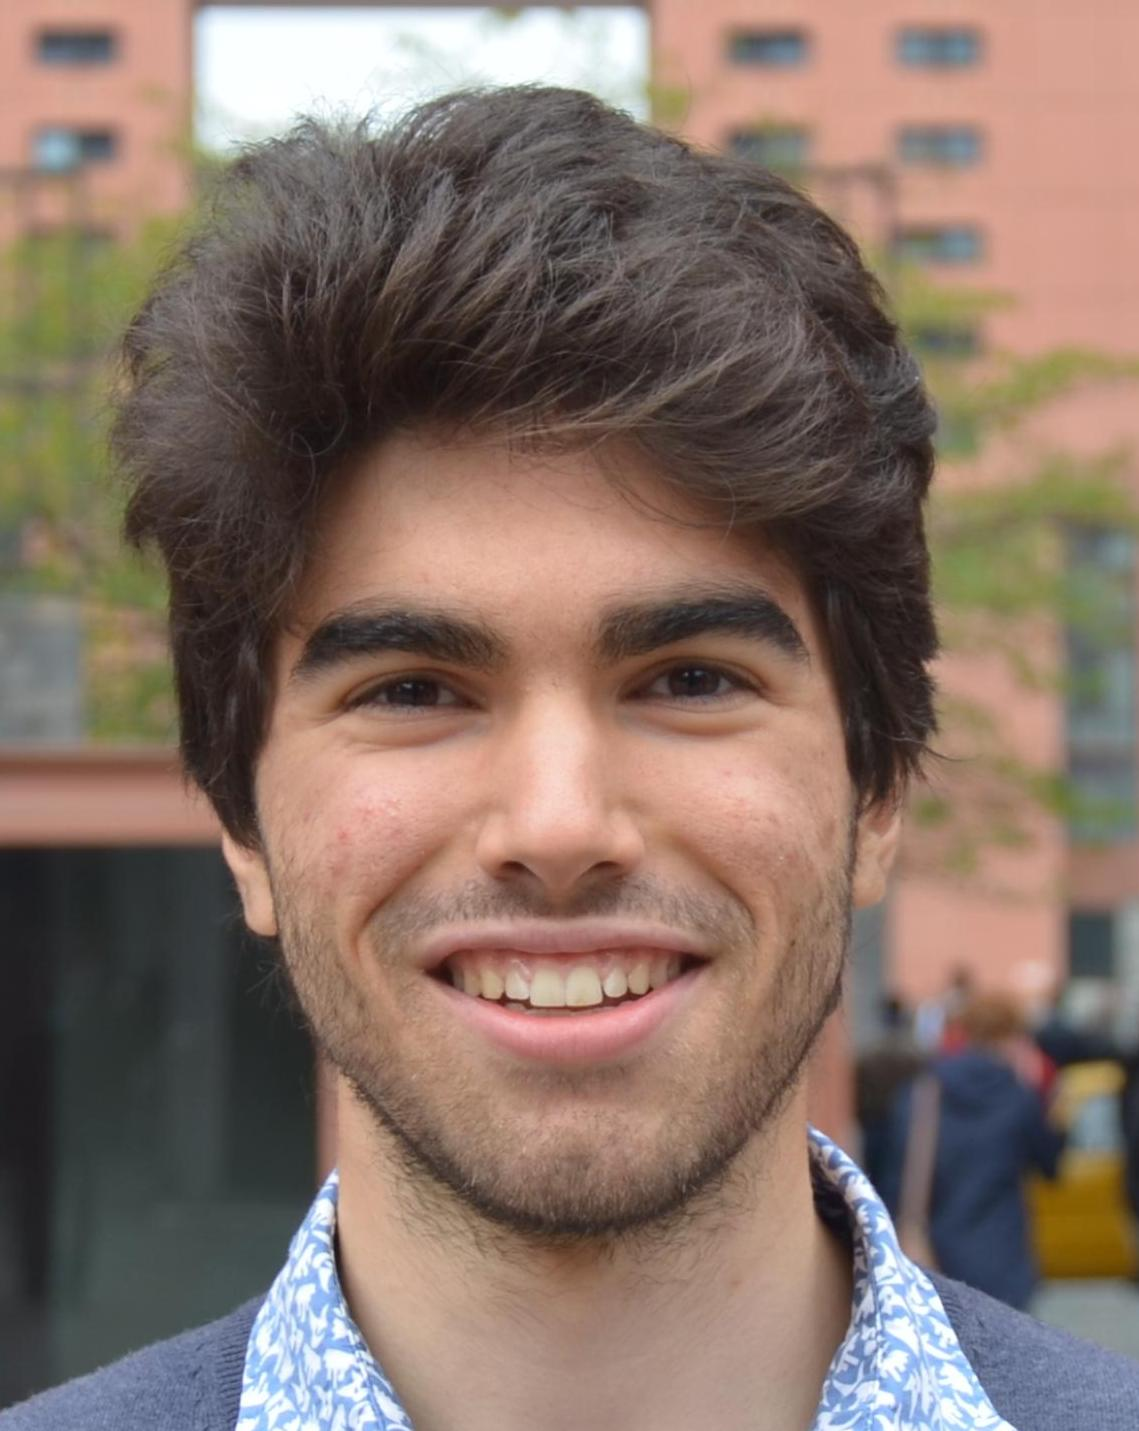
\includegraphics[width=0.1\linewidth]{Fototessera.jpg}}}

\noindent\spacedlowsmallcaps{Personal Information}\vspace{0.5em} % Personal information heading

\NewEntry{}{\textit{Born in Italy,}}{03 January 1997} % Birthplace and date

\NewEntry{email}{\href{mailto:apanontin@tutanota.com}{apanontin@tutanota.com}}% Email address

\NewEntry{phone}{(M) +39 348 533 7566\ \ $\cdotp$\ \ (M) +33 7 55 62 46 96} % Phone number(s)

\Description{\MarginText{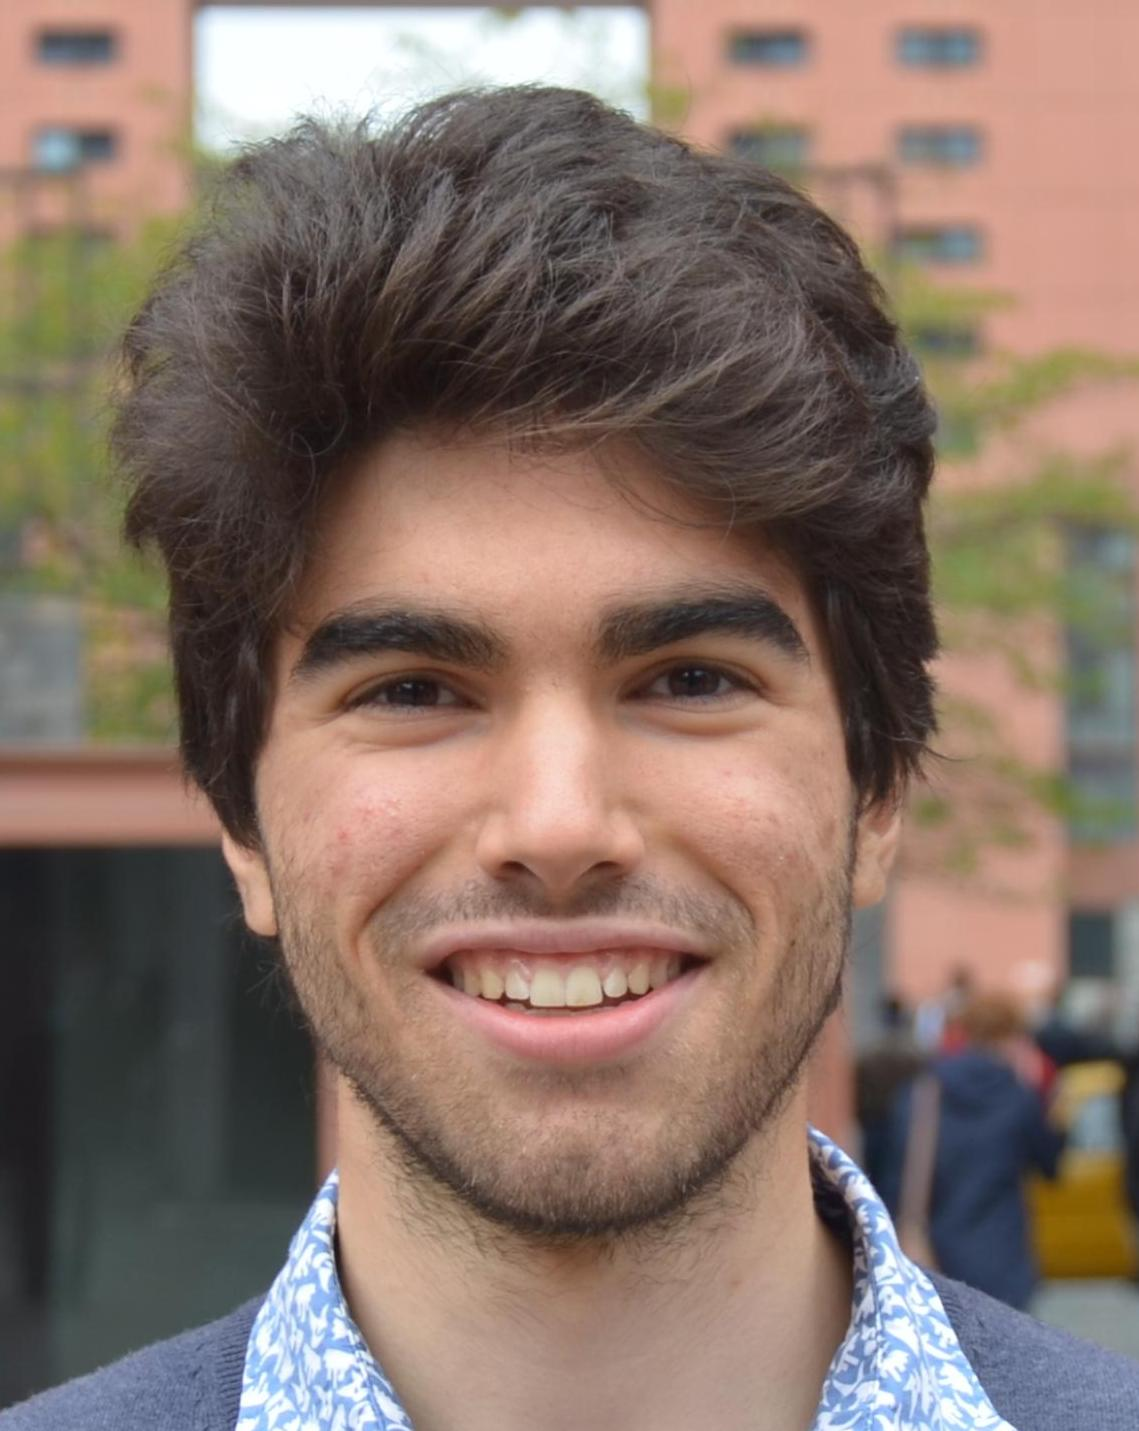
\includegraphics[width=\linewidth]{Fototessera.jpg}}}
\vspace{-1em} % Extra white space between the personal information section and goal

%----------------------------------------------------------------------------------------
%	EDUCATION
%----------------------------------------------------------------------------------------

\noindent\spacedlowsmallcaps{Education}\vspace{1em}

\NewEntry{2019-2021}{ALGANT Master Program}

\Description{\MarginText{Master of Mathematics}%Master degree focused on ALgebra,
%	Geometry and Number Theory.\newline
Mobility Scheme: Padova (1st year), Bordeaux (2nd year).\newline
Working on a thesis in $p$-adic Hodge theory,\newline
under the supervision of Professor Olivier Brinon.}

%------------------------------------------------

\NewEntry{2016-2019}{Università degli Studi di Milano-Bicocca}

\Description{\MarginText{Bachelor of Mathematics}Graduated in September 2019, grade: 110/110 e Lode.\newline
Thesis: {\em Introduction to quantum computing},\newline
under the supervision of Professor Davide L. Ferrario.}

%------------------------------------------------

\NewEntry{2011-2016}{Liceo Scientifico Statale ``Federigo Enriques''}

\Description{\MarginText{High School Diploma}Grade: 100/100.\newline 
Thesis: \textit{Macchine Pensanti: l'Ultima Sfida della Società Contemporanea}.}

%------------------------------------------------

\vspace{1em} % Extra space between major sections

%----------------------------------------------------------------------------------------
%	COMPUTER SKILLS
%----------------------------------------------------------------------------------------

\spacedlowsmallcaps{Skills}\vspace{1em}
%------------------------------------------------

%\vspace{1em}

\newlength{\langbox} % Create a new length for the length of languages to keep them equally spaced
\settowidth{\langbox}{English} % Length equals the length of "English" - if you have a longer language in your list put it here

\Description{\MarginText{Languages}\parbox{\langbox}{\textsc{Italian}}\ \ $\cdotp$\ \ \ Mothertongue}

\vspace{-0.5em} % Negative vertical space to counteract the vertical space between every \Description command

\Description{\parbox{\langbox}{\textsc{English}}\ \ $\cdotp$\ \ \ Fluent (8.0 IELTS score)}

\vspace{-0.5em} % Negative vertical space to counteract the vertical space between every \Description command

\Description{\parbox{\langbox}{\textsc{French}}\ \ $\cdotp$\ \ \ Basic (attending B1 course)}

%------------------------------------------------
\newlength{\skillbox} % Create a new length for the length of languages to keep them equally spaced
\settowidth{\skillbox}{Intermedia} 

\Description{\MarginText{Computer}\parbox{\skillbox}{Basic}\ \ $\cdotp$\ \ \ \textsc{sage}, \textsc{python}, \textsc{matlab}, git}

\vspace{-0.5em} % Negative vertical space to counteract the vertical space between every \Description command

\Description{\parbox{\skillbox}{Intermediate}\ \ $\cdotp$\ \ \ Linux/Unix, \textsc{oop java}, \LaTeX}

%\Description{\MarginText{Computer}Basic: .\newline
%Intermediate: }

%\Description{\MarginText{Advanced}Computer Hardware and Support}

%------------------------------------------------

\vspace{1em} % Extra space between major sections

%----------------------------------------------------------------------------------------
%	OTHER INFORMATION
%----------------------------------------------------------------------------------------

\spacedlowsmallcaps{Other Information}\vspace{1em}

\Description{\MarginText{Various}2009, 2011\ \ $\cdotp$\ \ Participation at national round of \textit{Campionati Internazionali di Giochi Matematici}.}

\vspace{-0.5em} % Negative vertical space to counteract the vertical space between every \Description command

\Description{2012-2016\ \ $\cdotp$\ \ Various participations at \textit{Olimpiadi della Matematica}.}

\vspace{-0.5em} % Negative vertical space to counteract the vertical space between every \Description command

\Description{2008-2017\ \ $\cdotp$\ \ Practiced Cycling at a competitive level, with various participations in international races, up to Under 23 level.}

%------------------------------------------------

\vspace{1em}

\Description{\MarginText{University Duties}2017 - 2019\ \ $\cdotp$\ \ Member of the Students' Representative Council,\\ 
Math Department Council and Math Didactic Council at Università degli Studi di Milano-Bicocca.}

\vspace{1em} % Negative vertical space to counteract the vertical space between every \Description command

%\noindent\spacedlowsmallcaps{Goal}\vspace{1em} % Goal heading, could be used for a quotation or short profile instead

\Description{\MarginText{Personal}The many years spent practising cycling
left me a passion for sport and nature, which I try to keep alive alongside my studies. %\newline
I am interested in all that concerns design and IT
and I try to fuel these interests in my everyday life.\newline
In mathematics I feel attracted to homological algebra
and $p$-adic Hodge theory.\\
For more (up to date) information see 
\href{https://github.com/andreapanontin}{https://github.com/andreapanontin}.}

%I am a meticulous and dedicated person,
%with a strong predisposition to practical thinking and problem solving.
%I am willing to enrich my knowledge and my competences in the topics
%I am interested in, among which mathematics, computer science and design.}
%\vspace{.1em} % Goal text

%------------------------------------------------

%\Description{\MarginText{Interests}Piano\ \ $\cdotp$\ \ Cooking\ \ $\cdotp$\ \ Running\ \ $\cdotp$\ \ Chess\ \ $\cdotp$\ \ Dancing}

%----------------------------------------------------------------------------------------

\end{cv}

\end{document}
